\documentclass[12pt]{article}
\usepackage{url,amsmath,amsthm,enumitem,amsfonts,tikz,verbatim,amssymb, wasysym, clrscode3e, booktabs, soul}
% \usepackage[doublespacing]{setspace}
\usepackage[makeroom]{cancel}
\usepackage{natbib}
\usepackage{graphicx}
\usepackage{listings}
\usetikzlibrary{arrows}

\title{ University of Massachusetts Lowell \protect\\
	Department of Mathematical Sciences\protect\\
MATH 4750 \protect\\
Senior Seminar Project Report}
\author{Joel Savitz \\ Fall 2020 \\ SID: 01739537}

\lstset
{
    %Formatting for code in appendix
    showstringspaces=false,
    breaklines=true,
    breakatwhitespace=false,
}

\newcommand{\reals}{\mathbb{R}}

\begin{document}

\maketitle

\begin{abstract}
//TODO
\end{abstract}

\section{Introduction}

Scientists express physical laws of
the universe in the language of differential equations.
The reason for this is not immediately obvious,
though my personal work with differential equations
has provided me with an intuition as to why.
Fortunately for me,
one scientist describes three necessary properties
of a physical law that are satisfied by a differential equation as: 


\begin{itemize}
	\item ``The mathematical relation must be sufficiently general"
	\item ``It must define connections between neighboring points"
	\item ``It must imply the continuity of change"\citep{whydiffeq}
\end{itemize}

Differential equations satisfy all three of these properties
since they are general enough that
changes to the initial values of a system
do not violate the constraints defined by a general solution
and the relationship between a function and one or more of its derivatives
defines the connection between points in the domain of the function
and implies that change in the system is continuous
due to the nature of calculus.


Newton's law of cooling states that
``the rate of heat loss of a body is
directly proportional to the difference
in the temperatures between the body and
its surroundings" \citep{wiki}.

Let $\Delta T$ be the difference between
the temperature of the body
and the ambient temperature of the environment
as a function of a point in time $t$,
we have that equation \ref{eq1}
describes Newton's law of cooling.

\begin{align} \label{eq1}
	\frac{d\Delta T}{dt} = k\Delta T(t) \textrm{ for some $k \in \reals$}
\end{align}

Then, we can solve this differential equation by separating the paramaters.

\begin{align} \label{eq2}
	\frac{dT}{dt}\frac{1}{\Delta T(t)} & = k \\
	\int \frac{dT}{dt}\frac{1}{\Delta T(t)} dt & = \int k dt \\
	\ln|\Delta T(t)| & = kt + C \textrm{ for some $C \in \reals$} \\
	e^{\ln | \Delta T(t) | } = & e^{kt + C} \\
	\label{eq3}
	\Delta T(t) = & De^{kt} \textrm{ where $D = e^C$ }
\end{align}

In this paper, I verify the this law
relative to a particular environment
and calculate an approximate value of the cooling coefficient
by fitting experimental data to equation \ref{eq3}.

\section{Materials and Methods}

I performed this experiment using
using a hardware sensor
to a Raspbery Pi computer.

I purchased the DS18D20,
a waterproof temperature sensor compatible with the Raspberry Pi.
These sensors are relatively innexpensive,
and I purchased a 5 pack for $\$12.98$ on Amazon \citep{Amazon}.



Figure \ref{fig2} 

\begin{figure}
	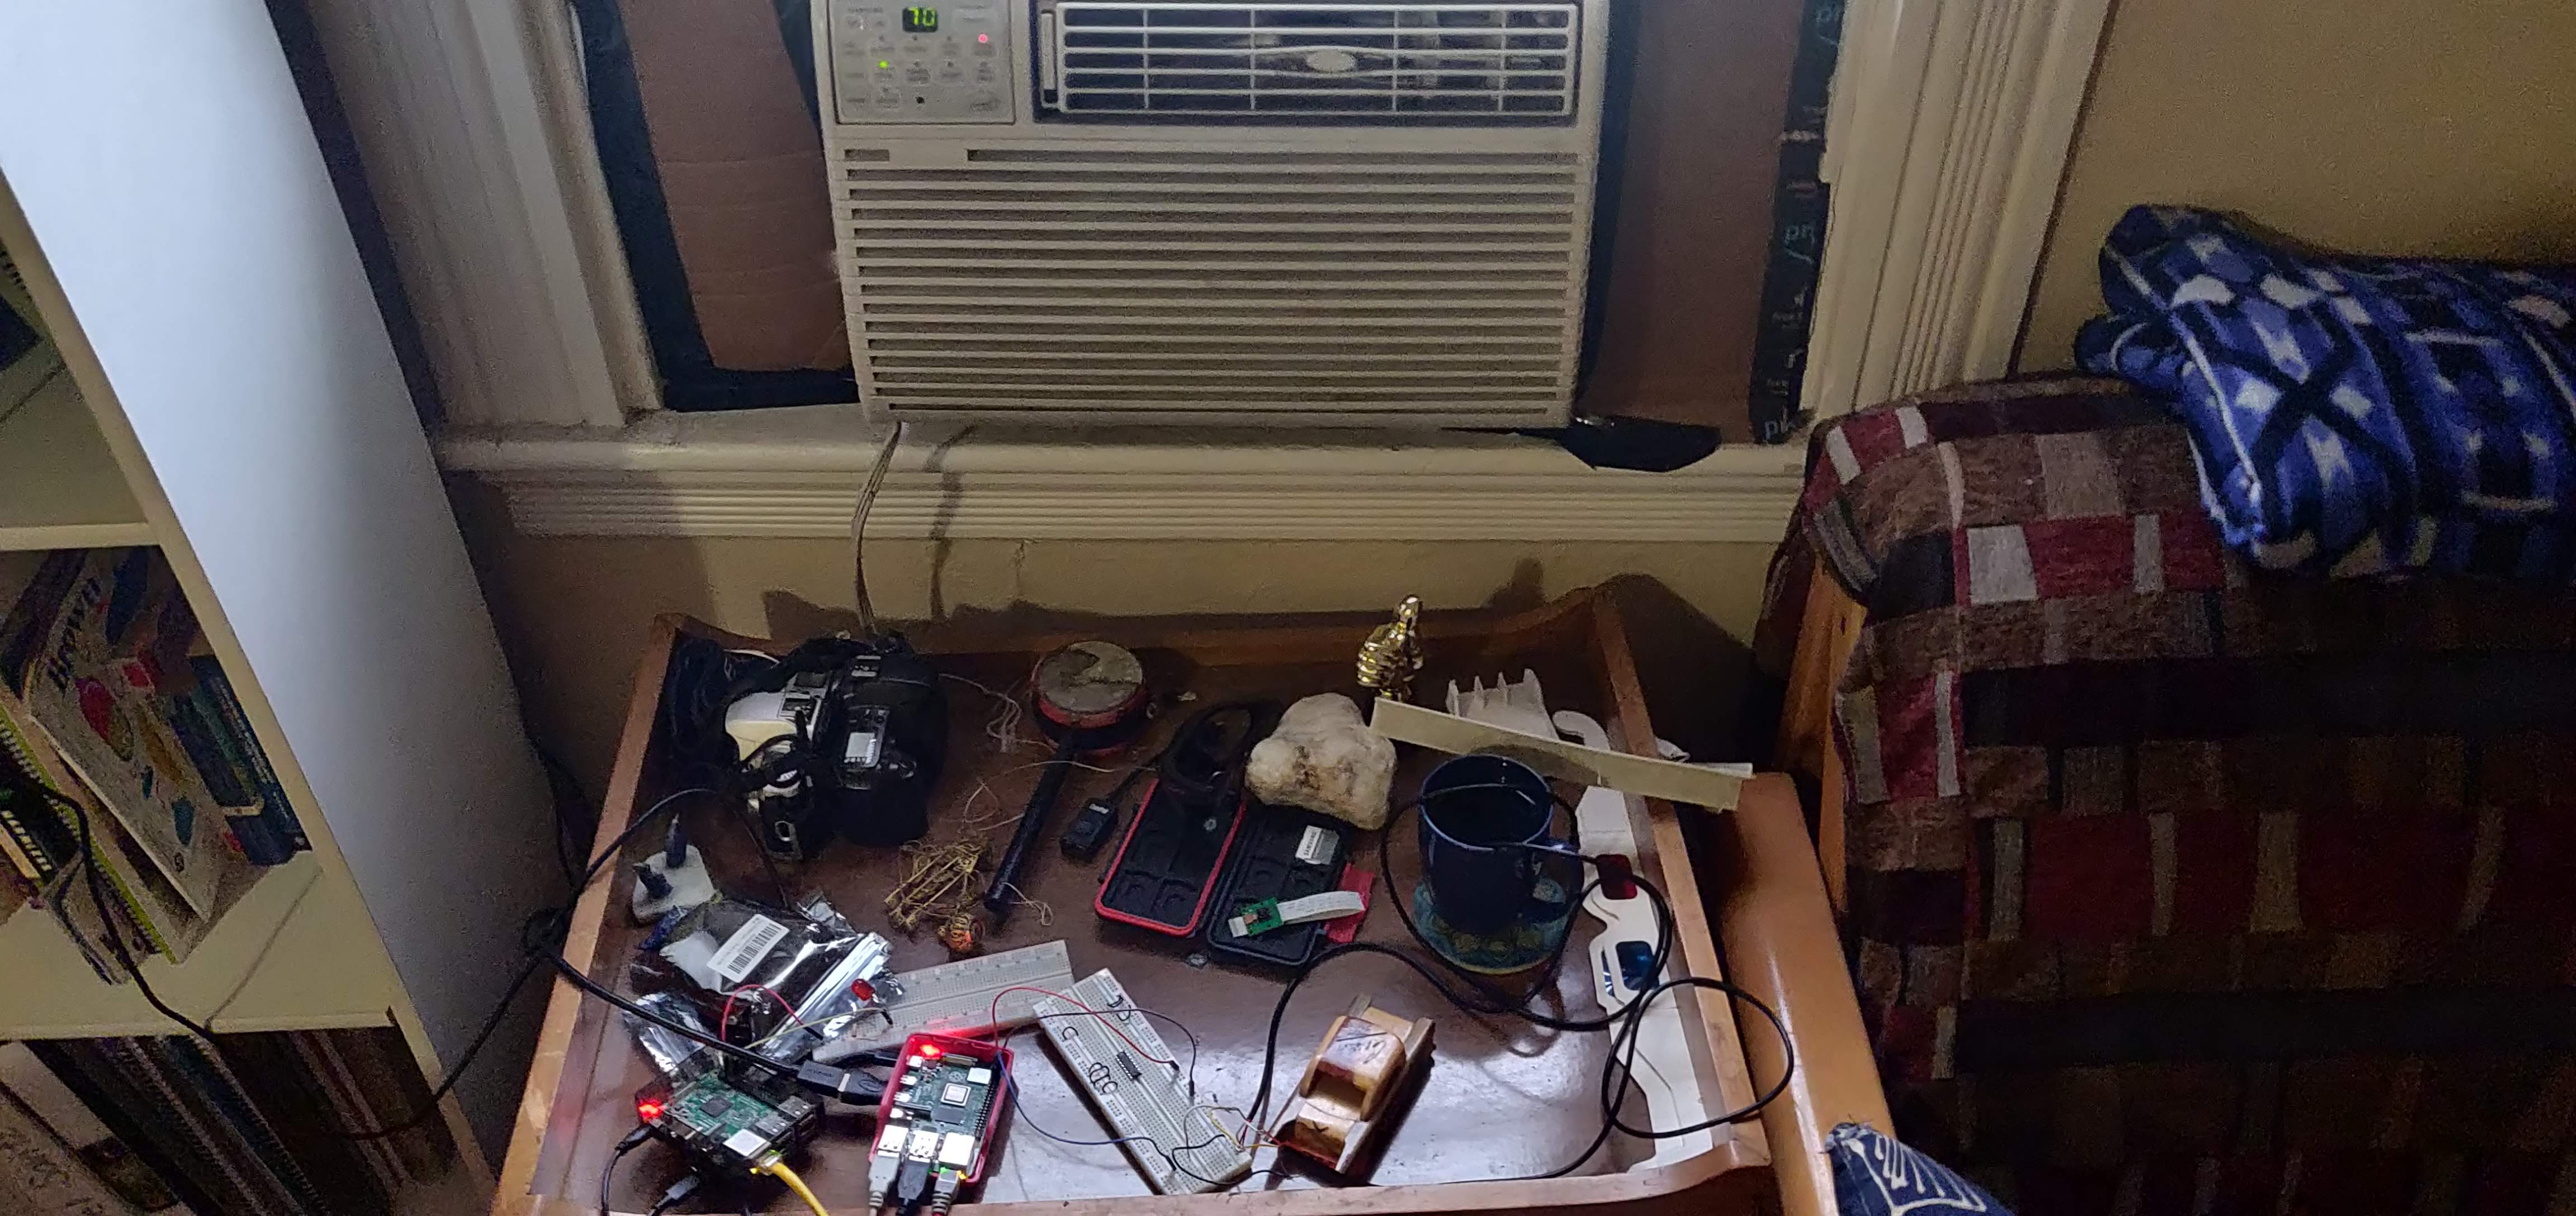
\includegraphics[scale=0.1]{full_setup.jpg}
	\centering
	\label{fig2}
	\caption{The full experimental setup}
\end{figure}

I wrote two programs to analyze the data.
See sections \ref{apxA} and \ref{apxB} for the full code listings.


\section{Results}

\begin{figure}
	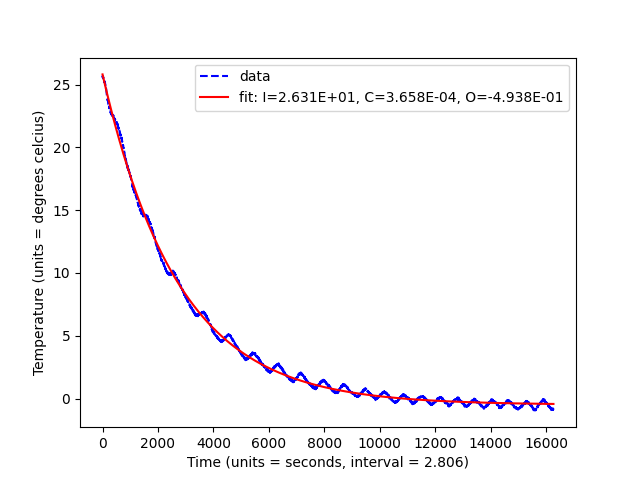
\includegraphics[scale=0.8]{Figure_1.png}
	\centering
	\label{fig1}
	\caption{A plot of the data and the fitted curve}
\end{figure}

\section{Discussion}

Newton was right lol

\section{Appendix A: The \texttt{gather} program} \label{apxA}

\subsection{Main program}

\lstinputlisting[language=Python]{../gather/gather.py}

\subsection{Wrapper shell script}

\lstinputlisting[language=bash]{../gather/gather.sh}

\section{Appendix B: The \texttt{analysis} program} \label{apxB}

\lstinputlisting[language=Python]{../analysis/analysis.py}

\bibliographystyle{unsrtnat}
\bibliography{timeline}

\end{document}
